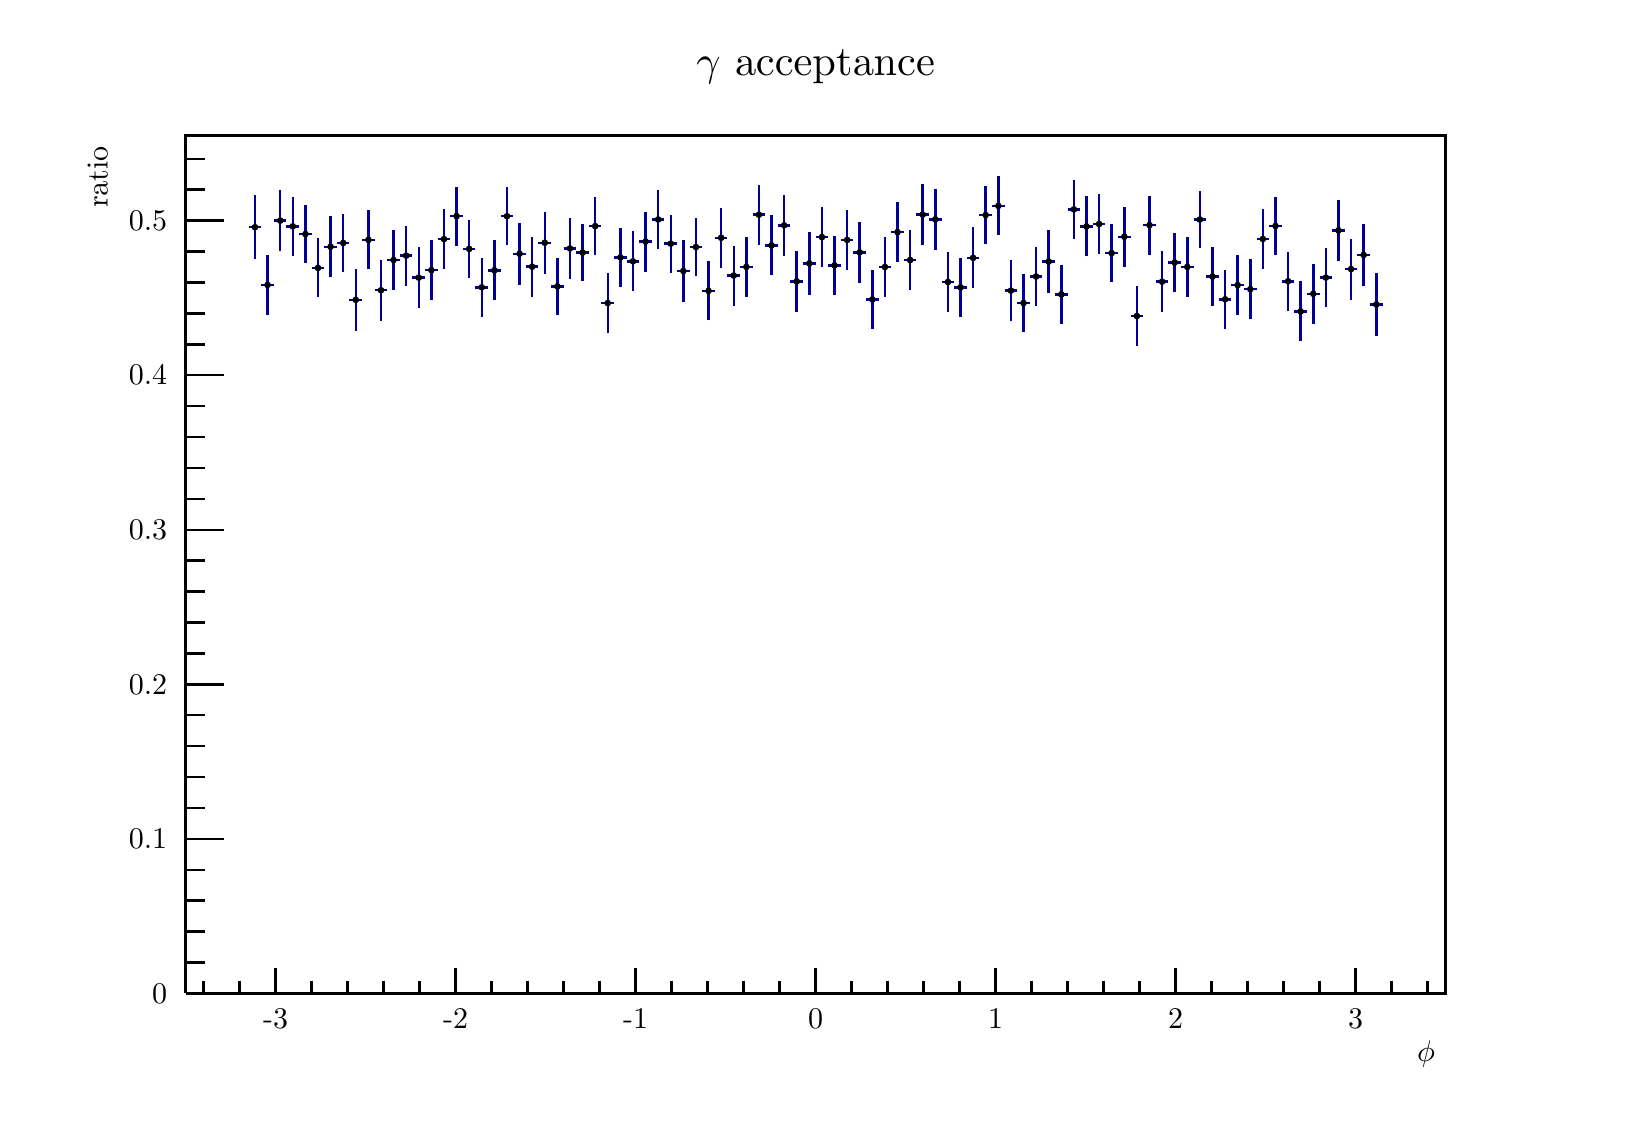
\begin{tikzpicture}
\pgfdeclareplotmark{cross} {
\pgfpathmoveto{\pgfpoint{-0.3\pgfplotmarksize}{\pgfplotmarksize}}
\pgfpathlineto{\pgfpoint{+0.3\pgfplotmarksize}{\pgfplotmarksize}}
\pgfpathlineto{\pgfpoint{+0.3\pgfplotmarksize}{0.3\pgfplotmarksize}}
\pgfpathlineto{\pgfpoint{+1\pgfplotmarksize}{0.3\pgfplotmarksize}}
\pgfpathlineto{\pgfpoint{+1\pgfplotmarksize}{-0.3\pgfplotmarksize}}
\pgfpathlineto{\pgfpoint{+0.3\pgfplotmarksize}{-0.3\pgfplotmarksize}}
\pgfpathlineto{\pgfpoint{+0.3\pgfplotmarksize}{-1.\pgfplotmarksize}}
\pgfpathlineto{\pgfpoint{-0.3\pgfplotmarksize}{-1.\pgfplotmarksize}}
\pgfpathlineto{\pgfpoint{-0.3\pgfplotmarksize}{-0.3\pgfplotmarksize}}
\pgfpathlineto{\pgfpoint{-1.\pgfplotmarksize}{-0.3\pgfplotmarksize}}
\pgfpathlineto{\pgfpoint{-1.\pgfplotmarksize}{0.3\pgfplotmarksize}}
\pgfpathlineto{\pgfpoint{-0.3\pgfplotmarksize}{0.3\pgfplotmarksize}}
\pgfpathclose
\pgfusepathqstroke
}
\pgfdeclareplotmark{cross*} {
\pgfpathmoveto{\pgfpoint{-0.3\pgfplotmarksize}{\pgfplotmarksize}}
\pgfpathlineto{\pgfpoint{+0.3\pgfplotmarksize}{\pgfplotmarksize}}
\pgfpathlineto{\pgfpoint{+0.3\pgfplotmarksize}{0.3\pgfplotmarksize}}
\pgfpathlineto{\pgfpoint{+1\pgfplotmarksize}{0.3\pgfplotmarksize}}
\pgfpathlineto{\pgfpoint{+1\pgfplotmarksize}{-0.3\pgfplotmarksize}}
\pgfpathlineto{\pgfpoint{+0.3\pgfplotmarksize}{-0.3\pgfplotmarksize}}
\pgfpathlineto{\pgfpoint{+0.3\pgfplotmarksize}{-1.\pgfplotmarksize}}
\pgfpathlineto{\pgfpoint{-0.3\pgfplotmarksize}{-1.\pgfplotmarksize}}
\pgfpathlineto{\pgfpoint{-0.3\pgfplotmarksize}{-0.3\pgfplotmarksize}}
\pgfpathlineto{\pgfpoint{-1.\pgfplotmarksize}{-0.3\pgfplotmarksize}}
\pgfpathlineto{\pgfpoint{-1.\pgfplotmarksize}{0.3\pgfplotmarksize}}
\pgfpathlineto{\pgfpoint{-0.3\pgfplotmarksize}{0.3\pgfplotmarksize}}
\pgfpathclose
\pgfusepathqfillstroke
}
\pgfdeclareplotmark{newstar} {
\pgfpathmoveto{\pgfqpoint{0pt}{\pgfplotmarksize}}
\pgfpathlineto{\pgfqpointpolar{44}{0.5\pgfplotmarksize}}
\pgfpathlineto{\pgfqpointpolar{18}{\pgfplotmarksize}}
\pgfpathlineto{\pgfqpointpolar{-20}{0.5\pgfplotmarksize}}
\pgfpathlineto{\pgfqpointpolar{-54}{\pgfplotmarksize}}
\pgfpathlineto{\pgfqpointpolar{-90}{0.5\pgfplotmarksize}}
\pgfpathlineto{\pgfqpointpolar{234}{\pgfplotmarksize}}
\pgfpathlineto{\pgfqpointpolar{198}{0.5\pgfplotmarksize}}
\pgfpathlineto{\pgfqpointpolar{162}{\pgfplotmarksize}}
\pgfpathlineto{\pgfqpointpolar{134}{0.5\pgfplotmarksize}}
\pgfpathclose
\pgfusepathqstroke
}
\pgfdeclareplotmark{newstar*} {
\pgfpathmoveto{\pgfqpoint{0pt}{\pgfplotmarksize}}
\pgfpathlineto{\pgfqpointpolar{44}{0.5\pgfplotmarksize}}
\pgfpathlineto{\pgfqpointpolar{18}{\pgfplotmarksize}}
\pgfpathlineto{\pgfqpointpolar{-20}{0.5\pgfplotmarksize}}
\pgfpathlineto{\pgfqpointpolar{-54}{\pgfplotmarksize}}
\pgfpathlineto{\pgfqpointpolar{-90}{0.5\pgfplotmarksize}}
\pgfpathlineto{\pgfqpointpolar{234}{\pgfplotmarksize}}
\pgfpathlineto{\pgfqpointpolar{198}{0.5\pgfplotmarksize}}
\pgfpathlineto{\pgfqpointpolar{162}{\pgfplotmarksize}}
\pgfpathlineto{\pgfqpointpolar{134}{0.5\pgfplotmarksize}}
\pgfpathclose
\pgfusepathqfillstroke
}
\definecolor{c}{rgb}{1,1,1};
\draw [color=c, fill=c] (0,0) rectangle (20,13.6207);
\draw [color=c, fill=c] (2,1.36207) rectangle (18,12.2586);
\definecolor{c}{rgb}{0,0,0};
\draw [c,line width=0.9] (2,1.36207) -- (2,12.2586) -- (18,12.2586) -- (18,1.36207) -- (2,1.36207);
\definecolor{c}{rgb}{1,1,1};
\draw [color=c, fill=c] (2,1.36207) rectangle (18,12.2586);
\definecolor{c}{rgb}{0,0,0};
\draw [c,line width=0.9] (2,1.36207) -- (2,12.2586) -- (18,12.2586) -- (18,1.36207) -- (2,1.36207);
\definecolor{c}{rgb}{0,0,0.6};
\draw [c,line width=0.9] (2.88,10.6867) -- (2.88,11.0932);
\draw [c,line width=0.9] (2.88,11.0932) -- (2.88,11.4997);
\draw [c,line width=0.9] (2.8,11.0932) -- (2.88,11.0932);
\draw [c,line width=0.9] (2.88,11.0932) -- (2.96,11.0932);
\definecolor{c}{rgb}{0,0,0};
\foreach \P in {(2.88,11.0932)}{\draw[mark options={color=c,fill=c},mark size=2.402402pt,mark=*,mark size=1pt] plot coordinates {\P};}
\definecolor{c}{rgb}{0,0,0.6};
\draw [c,line width=0.9] (3.04,9.98025) -- (3.04,10.3607);
\draw [c,line width=0.9] (3.04,10.3607) -- (3.04,10.7412);
\draw [c,line width=0.9] (2.96,10.3607) -- (3.04,10.3607);
\draw [c,line width=0.9] (3.04,10.3607) -- (3.12,10.3607);
\definecolor{c}{rgb}{0,0,0};
\foreach \P in {(3.04,10.3607)}{\draw[mark options={color=c,fill=c},mark size=2.402402pt,mark=*,mark size=1pt] plot coordinates {\P};}
\definecolor{c}{rgb}{0,0,0.6};
\draw [c,line width=0.9] (3.2,10.7948) -- (3.2,11.1774);
\draw [c,line width=0.9] (3.2,11.1774) -- (3.2,11.5601);
\draw [c,line width=0.9] (3.12,11.1774) -- (3.2,11.1774);
\draw [c,line width=0.9] (3.2,11.1774) -- (3.28,11.1774);
\definecolor{c}{rgb}{0,0,0};
\foreach \P in {(3.2,11.1774)}{\draw[mark options={color=c,fill=c},mark size=2.402402pt,mark=*,mark size=1pt] plot coordinates {\P};}
\definecolor{c}{rgb}{0,0,0.6};
\draw [c,line width=0.9] (3.36,10.7254) -- (3.36,11.1043);
\draw [c,line width=0.9] (3.36,11.1043) -- (3.36,11.4832);
\draw [c,line width=0.9] (3.28,11.1043) -- (3.36,11.1043);
\draw [c,line width=0.9] (3.36,11.1043) -- (3.44,11.1043);
\definecolor{c}{rgb}{0,0,0};
\foreach \P in {(3.36,11.1043)}{\draw[mark options={color=c,fill=c},mark size=2.402402pt,mark=*,mark size=1pt] plot coordinates {\P};}
\definecolor{c}{rgb}{0,0,0.6};
\draw [c,line width=0.9] (3.52,10.6331) -- (3.52,11.0067);
\draw [c,line width=0.9] (3.52,11.0067) -- (3.52,11.3803);
\draw [c,line width=0.9] (3.44,11.0067) -- (3.52,11.0067);
\draw [c,line width=0.9] (3.52,11.0067) -- (3.6,11.0067);
\definecolor{c}{rgb}{0,0,0};
\foreach \P in {(3.52,11.0067)}{\draw[mark options={color=c,fill=c},mark size=2.402402pt,mark=*,mark size=1pt] plot coordinates {\P};}
\definecolor{c}{rgb}{0,0,0.6};
\draw [c,line width=0.9] (3.68,10.2024) -- (3.68,10.5765);
\draw [c,line width=0.9] (3.68,10.5765) -- (3.68,10.9505);
\draw [c,line width=0.9] (3.6,10.5765) -- (3.68,10.5765);
\draw [c,line width=0.9] (3.68,10.5765) -- (3.76,10.5765);
\definecolor{c}{rgb}{0,0,0};
\foreach \P in {(3.68,10.5765)}{\draw[mark options={color=c,fill=c},mark size=2.402402pt,mark=*,mark size=1pt] plot coordinates {\P};}
\definecolor{c}{rgb}{0,0,0.6};
\draw [c,line width=0.9] (3.84,10.4604) -- (3.84,10.8452);
\draw [c,line width=0.9] (3.84,10.8452) -- (3.84,11.23);
\draw [c,line width=0.9] (3.76,10.8452) -- (3.84,10.8452);
\draw [c,line width=0.9] (3.84,10.8452) -- (3.92,10.8452);
\definecolor{c}{rgb}{0,0,0};
\foreach \P in {(3.84,10.8452)}{\draw[mark options={color=c,fill=c},mark size=2.402402pt,mark=*,mark size=1pt] plot coordinates {\P};}
\definecolor{c}{rgb}{0,0,0.6};
\draw [c,line width=0.9] (4,10.5194) -- (4,10.8929);
\draw [c,line width=0.9] (4,10.8929) -- (4,11.2664);
\draw [c,line width=0.9] (3.92,10.8929) -- (4,10.8929);
\draw [c,line width=0.9] (4,10.8929) -- (4.08,10.8929);
\definecolor{c}{rgb}{0,0,0};
\foreach \P in {(4,10.8929)}{\draw[mark options={color=c,fill=c},mark size=2.402402pt,mark=*,mark size=1pt] plot coordinates {\P};}
\definecolor{c}{rgb}{0,0,0.6};
\draw [c,line width=0.9] (4.16,9.77985) -- (4.16,10.1707);
\draw [c,line width=0.9] (4.16,10.1707) -- (4.16,10.5616);
\draw [c,line width=0.9] (4.08,10.1707) -- (4.16,10.1707);
\draw [c,line width=0.9] (4.16,10.1707) -- (4.24,10.1707);
\definecolor{c}{rgb}{0,0,0};
\foreach \P in {(4.16,10.1707)}{\draw[mark options={color=c,fill=c},mark size=2.402402pt,mark=*,mark size=1pt] plot coordinates {\P};}
\definecolor{c}{rgb}{0,0,0.6};
\draw [c,line width=0.9] (4.32,10.5564) -- (4.32,10.9324);
\draw [c,line width=0.9] (4.32,10.9324) -- (4.32,11.3084);
\draw [c,line width=0.9] (4.24,10.9324) -- (4.32,10.9324);
\draw [c,line width=0.9] (4.32,10.9324) -- (4.4,10.9324);
\definecolor{c}{rgb}{0,0,0};
\foreach \P in {(4.32,10.9324)}{\draw[mark options={color=c,fill=c},mark size=2.402402pt,mark=*,mark size=1pt] plot coordinates {\P};}
\definecolor{c}{rgb}{0,0,0.6};
\draw [c,line width=0.9] (4.48,9.90821) -- (4.48,10.2934);
\draw [c,line width=0.9] (4.48,10.2934) -- (4.48,10.6786);
\draw [c,line width=0.9] (4.4,10.2934) -- (4.48,10.2934);
\draw [c,line width=0.9] (4.48,10.2934) -- (4.56,10.2934);
\definecolor{c}{rgb}{0,0,0};
\foreach \P in {(4.48,10.2934)}{\draw[mark options={color=c,fill=c},mark size=2.402402pt,mark=*,mark size=1pt] plot coordinates {\P};}
\definecolor{c}{rgb}{0,0,0.6};
\draw [c,line width=0.9] (4.64,10.2914) -- (4.64,10.6768);
\draw [c,line width=0.9] (4.64,10.6768) -- (4.64,11.0622);
\draw [c,line width=0.9] (4.56,10.6768) -- (4.64,10.6768);
\draw [c,line width=0.9] (4.64,10.6768) -- (4.72,10.6768);
\definecolor{c}{rgb}{0,0,0};
\foreach \P in {(4.64,10.6768)}{\draw[mark options={color=c,fill=c},mark size=2.402402pt,mark=*,mark size=1pt] plot coordinates {\P};}
\definecolor{c}{rgb}{0,0,0.6};
\draw [c,line width=0.9] (4.8,10.3515) -- (4.8,10.7326);
\draw [c,line width=0.9] (4.8,10.7326) -- (4.8,11.1137);
\draw [c,line width=0.9] (4.72,10.7326) -- (4.8,10.7326);
\draw [c,line width=0.9] (4.8,10.7326) -- (4.88,10.7326);
\definecolor{c}{rgb}{0,0,0};
\foreach \P in {(4.8,10.7326)}{\draw[mark options={color=c,fill=c},mark size=2.402402pt,mark=*,mark size=1pt] plot coordinates {\P};}
\definecolor{c}{rgb}{0,0,0.6};
\draw [c,line width=0.9] (4.96,10.0654) -- (4.96,10.4532);
\draw [c,line width=0.9] (4.96,10.4532) -- (4.96,10.841);
\draw [c,line width=0.9] (4.88,10.4532) -- (4.96,10.4532);
\draw [c,line width=0.9] (4.96,10.4532) -- (5.04,10.4532);
\definecolor{c}{rgb}{0,0,0};
\foreach \P in {(4.96,10.4532)}{\draw[mark options={color=c,fill=c},mark size=2.402402pt,mark=*,mark size=1pt] plot coordinates {\P};}
\definecolor{c}{rgb}{0,0,0.6};
\draw [c,line width=0.9] (5.12,10.1703) -- (5.12,10.5484);
\draw [c,line width=0.9] (5.12,10.5484) -- (5.12,10.9265);
\draw [c,line width=0.9] (5.04,10.5484) -- (5.12,10.5484);
\draw [c,line width=0.9] (5.12,10.5484) -- (5.2,10.5484);
\definecolor{c}{rgb}{0,0,0};
\foreach \P in {(5.12,10.5484)}{\draw[mark options={color=c,fill=c},mark size=2.402402pt,mark=*,mark size=1pt] plot coordinates {\P};}
\definecolor{c}{rgb}{0,0,0.6};
\draw [c,line width=0.9] (5.28,10.5627) -- (5.28,10.9423);
\draw [c,line width=0.9] (5.28,10.9423) -- (5.28,11.322);
\draw [c,line width=0.9] (5.2,10.9423) -- (5.28,10.9423);
\draw [c,line width=0.9] (5.28,10.9423) -- (5.36,10.9423);
\definecolor{c}{rgb}{0,0,0};
\foreach \P in {(5.28,10.9423)}{\draw[mark options={color=c,fill=c},mark size=2.402402pt,mark=*,mark size=1pt] plot coordinates {\P};}
\definecolor{c}{rgb}{0,0,0.6};
\draw [c,line width=0.9] (5.44,10.8603) -- (5.44,11.2345);
\draw [c,line width=0.9] (5.44,11.2345) -- (5.44,11.6087);
\draw [c,line width=0.9] (5.36,11.2345) -- (5.44,11.2345);
\draw [c,line width=0.9] (5.44,11.2345) -- (5.52,11.2345);
\definecolor{c}{rgb}{0,0,0};
\foreach \P in {(5.44,11.2345)}{\draw[mark options={color=c,fill=c},mark size=2.402402pt,mark=*,mark size=1pt] plot coordinates {\P};}
\definecolor{c}{rgb}{0,0,0.6};
\draw [c,line width=0.9] (5.6,10.4499) -- (5.6,10.818);
\draw [c,line width=0.9] (5.6,10.818) -- (5.6,11.1861);
\draw [c,line width=0.9] (5.52,10.818) -- (5.6,10.818);
\draw [c,line width=0.9] (5.6,10.818) -- (5.68,10.818);
\definecolor{c}{rgb}{0,0,0};
\foreach \P in {(5.6,10.818)}{\draw[mark options={color=c,fill=c},mark size=2.402402pt,mark=*,mark size=1pt] plot coordinates {\P};}
\definecolor{c}{rgb}{0,0,0.6};
\draw [c,line width=0.9] (5.76,9.95303) -- (5.76,10.3303);
\draw [c,line width=0.9] (5.76,10.3303) -- (5.76,10.7075);
\draw [c,line width=0.9] (5.68,10.3303) -- (5.76,10.3303);
\draw [c,line width=0.9] (5.76,10.3303) -- (5.84,10.3303);
\definecolor{c}{rgb}{0,0,0};
\foreach \P in {(5.76,10.3303)}{\draw[mark options={color=c,fill=c},mark size=2.402402pt,mark=*,mark size=1pt] plot coordinates {\P};}
\definecolor{c}{rgb}{0,0,0.6};
\draw [c,line width=0.9] (5.92,10.1678) -- (5.92,10.5465);
\draw [c,line width=0.9] (5.92,10.5465) -- (5.92,10.9252);
\draw [c,line width=0.9] (5.84,10.5465) -- (5.92,10.5465);
\draw [c,line width=0.9] (5.92,10.5465) -- (6,10.5465);
\definecolor{c}{rgb}{0,0,0};
\foreach \P in {(5.92,10.5465)}{\draw[mark options={color=c,fill=c},mark size=2.402402pt,mark=*,mark size=1pt] plot coordinates {\P};}
\definecolor{c}{rgb}{0,0,0.6};
\draw [c,line width=0.9] (6.08,10.8625) -- (6.08,11.2335);
\draw [c,line width=0.9] (6.08,11.2335) -- (6.08,11.6045);
\draw [c,line width=0.9] (6,11.2335) -- (6.08,11.2335);
\draw [c,line width=0.9] (6.08,11.2335) -- (6.16,11.2335);
\definecolor{c}{rgb}{0,0,0};
\foreach \P in {(6.08,11.2335)}{\draw[mark options={color=c,fill=c},mark size=2.402402pt,mark=*,mark size=1pt] plot coordinates {\P};}
\definecolor{c}{rgb}{0,0,0.6};
\draw [c,line width=0.9] (6.24,10.3651) -- (6.24,10.7561);
\draw [c,line width=0.9] (6.24,10.7561) -- (6.24,11.1471);
\draw [c,line width=0.9] (6.16,10.7561) -- (6.24,10.7561);
\draw [c,line width=0.9] (6.24,10.7561) -- (6.32,10.7561);
\definecolor{c}{rgb}{0,0,0};
\foreach \P in {(6.24,10.7561)}{\draw[mark options={color=c,fill=c},mark size=2.402402pt,mark=*,mark size=1pt] plot coordinates {\P};}
\definecolor{c}{rgb}{0,0,0.6};
\draw [c,line width=0.9] (6.4,10.2129) -- (6.4,10.5914);
\draw [c,line width=0.9] (6.4,10.5914) -- (6.4,10.9699);
\draw [c,line width=0.9] (6.32,10.5914) -- (6.4,10.5914);
\draw [c,line width=0.9] (6.4,10.5914) -- (6.48,10.5914);
\definecolor{c}{rgb}{0,0,0};
\foreach \P in {(6.4,10.5914)}{\draw[mark options={color=c,fill=c},mark size=2.402402pt,mark=*,mark size=1pt] plot coordinates {\P};}
\definecolor{c}{rgb}{0,0,0.6};
\draw [c,line width=0.9] (6.56,10.5046) -- (6.56,10.8961);
\draw [c,line width=0.9] (6.56,10.8961) -- (6.56,11.2876);
\draw [c,line width=0.9] (6.48,10.8961) -- (6.56,10.8961);
\draw [c,line width=0.9] (6.56,10.8961) -- (6.64,10.8961);
\definecolor{c}{rgb}{0,0,0};
\foreach \P in {(6.56,10.8961)}{\draw[mark options={color=c,fill=c},mark size=2.402402pt,mark=*,mark size=1pt] plot coordinates {\P};}
\definecolor{c}{rgb}{0,0,0.6};
\draw [c,line width=0.9] (6.72,9.97712) -- (6.72,10.3424);
\draw [c,line width=0.9] (6.72,10.3424) -- (6.72,10.7076);
\draw [c,line width=0.9] (6.64,10.3424) -- (6.72,10.3424);
\draw [c,line width=0.9] (6.72,10.3424) -- (6.8,10.3424);
\definecolor{c}{rgb}{0,0,0};
\foreach \P in {(6.72,10.3424)}{\draw[mark options={color=c,fill=c},mark size=2.402402pt,mark=*,mark size=1pt] plot coordinates {\P};}
\definecolor{c}{rgb}{0,0,0.6};
\draw [c,line width=0.9] (6.88,10.4361) -- (6.88,10.8241);
\draw [c,line width=0.9] (6.88,10.8241) -- (6.88,11.2122);
\draw [c,line width=0.9] (6.8,10.8241) -- (6.88,10.8241);
\draw [c,line width=0.9] (6.88,10.8241) -- (6.96,10.8241);
\definecolor{c}{rgb}{0,0,0};
\foreach \P in {(6.88,10.8241)}{\draw[mark options={color=c,fill=c},mark size=2.402402pt,mark=*,mark size=1pt] plot coordinates {\P};}
\definecolor{c}{rgb}{0,0,0.6};
\draw [c,line width=0.9] (7.04,10.4078) -- (7.04,10.7718);
\draw [c,line width=0.9] (7.04,10.7718) -- (7.04,11.1358);
\draw [c,line width=0.9] (6.96,10.7718) -- (7.04,10.7718);
\draw [c,line width=0.9] (7.04,10.7718) -- (7.12,10.7718);
\definecolor{c}{rgb}{0,0,0};
\foreach \P in {(7.04,10.7718)}{\draw[mark options={color=c,fill=c},mark size=2.402402pt,mark=*,mark size=1pt] plot coordinates {\P};}
\definecolor{c}{rgb}{0,0,0.6};
\draw [c,line width=0.9] (7.2,10.736) -- (7.2,11.1072);
\draw [c,line width=0.9] (7.2,11.1072) -- (7.2,11.4784);
\draw [c,line width=0.9] (7.12,11.1072) -- (7.2,11.1072);
\draw [c,line width=0.9] (7.2,11.1072) -- (7.28,11.1072);
\definecolor{c}{rgb}{0,0,0};
\foreach \P in {(7.2,11.1072)}{\draw[mark options={color=c,fill=c},mark size=2.402402pt,mark=*,mark size=1pt] plot coordinates {\P};}
\definecolor{c}{rgb}{0,0,0.6};
\draw [c,line width=0.9] (7.36,9.749) -- (7.36,10.13);
\draw [c,line width=0.9] (7.36,10.13) -- (7.36,10.5111);
\draw [c,line width=0.9] (7.28,10.13) -- (7.36,10.13);
\draw [c,line width=0.9] (7.36,10.13) -- (7.44,10.13);
\definecolor{c}{rgb}{0,0,0};
\foreach \P in {(7.36,10.13)}{\draw[mark options={color=c,fill=c},mark size=2.402402pt,mark=*,mark size=1pt] plot coordinates {\P};}
\definecolor{c}{rgb}{0,0,0.6};
\draw [c,line width=0.9] (7.52,10.3318) -- (7.52,10.71);
\draw [c,line width=0.9] (7.52,10.71) -- (7.52,11.0882);
\draw [c,line width=0.9] (7.44,10.71) -- (7.52,10.71);
\draw [c,line width=0.9] (7.52,10.71) -- (7.6,10.71);
\definecolor{c}{rgb}{0,0,0};
\foreach \P in {(7.52,10.71)}{\draw[mark options={color=c,fill=c},mark size=2.402402pt,mark=*,mark size=1pt] plot coordinates {\P};}
\definecolor{c}{rgb}{0,0,0.6};
\draw [c,line width=0.9] (7.68,10.2807) -- (7.68,10.6608);
\draw [c,line width=0.9] (7.68,10.6608) -- (7.68,11.0409);
\draw [c,line width=0.9] (7.6,10.6608) -- (7.68,10.6608);
\draw [c,line width=0.9] (7.68,10.6608) -- (7.76,10.6608);
\definecolor{c}{rgb}{0,0,0};
\foreach \P in {(7.68,10.6608)}{\draw[mark options={color=c,fill=c},mark size=2.402402pt,mark=*,mark size=1pt] plot coordinates {\P};}
\definecolor{c}{rgb}{0,0,0.6};
\draw [c,line width=0.9] (7.84,10.5306) -- (7.84,10.9113);
\draw [c,line width=0.9] (7.84,10.9113) -- (7.84,11.2921);
\draw [c,line width=0.9] (7.76,10.9113) -- (7.84,10.9113);
\draw [c,line width=0.9] (7.84,10.9113) -- (7.92,10.9113);
\definecolor{c}{rgb}{0,0,0};
\foreach \P in {(7.84,10.9113)}{\draw[mark options={color=c,fill=c},mark size=2.402402pt,mark=*,mark size=1pt] plot coordinates {\P};}
\definecolor{c}{rgb}{0,0,0.6};
\draw [c,line width=0.9] (8,10.8192) -- (8,11.1915);
\draw [c,line width=0.9] (8,11.1915) -- (8,11.5638);
\draw [c,line width=0.9] (7.92,11.1915) -- (8,11.1915);
\draw [c,line width=0.9] (8,11.1915) -- (8.08,11.1915);
\definecolor{c}{rgb}{0,0,0};
\foreach \P in {(8,11.1915)}{\draw[mark options={color=c,fill=c},mark size=2.402402pt,mark=*,mark size=1pt] plot coordinates {\P};}
\definecolor{c}{rgb}{0,0,0.6};
\draw [c,line width=0.9] (8.16,10.5142) -- (8.16,10.8842);
\draw [c,line width=0.9] (8.16,10.8842) -- (8.16,11.2542);
\draw [c,line width=0.9] (8.08,10.8842) -- (8.16,10.8842);
\draw [c,line width=0.9] (8.16,10.8842) -- (8.24,10.8842);
\definecolor{c}{rgb}{0,0,0};
\foreach \P in {(8.16,10.8842)}{\draw[mark options={color=c,fill=c},mark size=2.402402pt,mark=*,mark size=1pt] plot coordinates {\P};}
\definecolor{c}{rgb}{0,0,0.6};
\draw [c,line width=0.9] (8.32,10.1471) -- (8.32,10.5376);
\draw [c,line width=0.9] (8.32,10.5376) -- (8.32,10.9281);
\draw [c,line width=0.9] (8.24,10.5376) -- (8.32,10.5376);
\draw [c,line width=0.9] (8.32,10.5376) -- (8.4,10.5376);
\definecolor{c}{rgb}{0,0,0};
\foreach \P in {(8.32,10.5376)}{\draw[mark options={color=c,fill=c},mark size=2.402402pt,mark=*,mark size=1pt] plot coordinates {\P};}
\definecolor{c}{rgb}{0,0,0.6};
\draw [c,line width=0.9] (8.48,10.4716) -- (8.48,10.8418);
\draw [c,line width=0.9] (8.48,10.8418) -- (8.48,11.2121);
\draw [c,line width=0.9] (8.4,10.8418) -- (8.48,10.8418);
\draw [c,line width=0.9] (8.48,10.8418) -- (8.56,10.8418);
\definecolor{c}{rgb}{0,0,0};
\foreach \P in {(8.48,10.8418)}{\draw[mark options={color=c,fill=c},mark size=2.402402pt,mark=*,mark size=1pt] plot coordinates {\P};}
\definecolor{c}{rgb}{0,0,0.6};
\draw [c,line width=0.9] (8.64,9.91081) -- (8.64,10.2851);
\draw [c,line width=0.9] (8.64,10.2851) -- (8.64,10.6594);
\draw [c,line width=0.9] (8.56,10.2851) -- (8.64,10.2851);
\draw [c,line width=0.9] (8.64,10.2851) -- (8.72,10.2851);
\definecolor{c}{rgb}{0,0,0};
\foreach \P in {(8.64,10.2851)}{\draw[mark options={color=c,fill=c},mark size=2.402402pt,mark=*,mark size=1pt] plot coordinates {\P};}
\definecolor{c}{rgb}{0,0,0.6};
\draw [c,line width=0.9] (8.8,10.5804) -- (8.8,10.9586);
\draw [c,line width=0.9] (8.8,10.9586) -- (8.8,11.3369);
\draw [c,line width=0.9] (8.72,10.9586) -- (8.8,10.9586);
\draw [c,line width=0.9] (8.8,10.9586) -- (8.88,10.9586);
\definecolor{c}{rgb}{0,0,0};
\foreach \P in {(8.8,10.9586)}{\draw[mark options={color=c,fill=c},mark size=2.402402pt,mark=*,mark size=1pt] plot coordinates {\P};}
\definecolor{c}{rgb}{0,0,0.6};
\draw [c,line width=0.9] (8.96,10.0987) -- (8.96,10.4795);
\draw [c,line width=0.9] (8.96,10.4795) -- (8.96,10.8603);
\draw [c,line width=0.9] (8.88,10.4795) -- (8.96,10.4795);
\draw [c,line width=0.9] (8.96,10.4795) -- (9.04,10.4795);
\definecolor{c}{rgb}{0,0,0};
\foreach \P in {(8.96,10.4795)}{\draw[mark options={color=c,fill=c},mark size=2.402402pt,mark=*,mark size=1pt] plot coordinates {\P};}
\definecolor{c}{rgb}{0,0,0.6};
\draw [c,line width=0.9] (9.12,10.2106) -- (9.12,10.5897);
\draw [c,line width=0.9] (9.12,10.5897) -- (9.12,10.9688);
\draw [c,line width=0.9] (9.04,10.5897) -- (9.12,10.5897);
\draw [c,line width=0.9] (9.12,10.5897) -- (9.2,10.5897);
\definecolor{c}{rgb}{0,0,0};
\foreach \P in {(9.12,10.5897)}{\draw[mark options={color=c,fill=c},mark size=2.402402pt,mark=*,mark size=1pt] plot coordinates {\P};}
\definecolor{c}{rgb}{0,0,0.6};
\draw [c,line width=0.9] (9.28,10.8692) -- (9.28,11.2521);
\draw [c,line width=0.9] (9.28,11.2521) -- (9.28,11.635);
\draw [c,line width=0.9] (9.2,11.2521) -- (9.28,11.2521);
\draw [c,line width=0.9] (9.28,11.2521) -- (9.36,11.2521);
\definecolor{c}{rgb}{0,0,0};
\foreach \P in {(9.28,11.2521)}{\draw[mark options={color=c,fill=c},mark size=2.402402pt,mark=*,mark size=1pt] plot coordinates {\P};}
\definecolor{c}{rgb}{0,0,0.6};
\draw [c,line width=0.9] (9.44,10.4809) -- (9.44,10.8637);
\draw [c,line width=0.9] (9.44,10.8637) -- (9.44,11.2464);
\draw [c,line width=0.9] (9.36,10.8637) -- (9.44,10.8637);
\draw [c,line width=0.9] (9.44,10.8637) -- (9.52,10.8637);
\definecolor{c}{rgb}{0,0,0};
\foreach \P in {(9.44,10.8637)}{\draw[mark options={color=c,fill=c},mark size=2.402402pt,mark=*,mark size=1pt] plot coordinates {\P};}
\definecolor{c}{rgb}{0,0,0.6};
\draw [c,line width=0.9] (9.6,10.7328) -- (9.6,11.1172);
\draw [c,line width=0.9] (9.6,11.1172) -- (9.6,11.5016);
\draw [c,line width=0.9] (9.52,11.1172) -- (9.6,11.1172);
\draw [c,line width=0.9] (9.6,11.1172) -- (9.68,11.1172);
\definecolor{c}{rgb}{0,0,0};
\foreach \P in {(9.6,11.1172)}{\draw[mark options={color=c,fill=c},mark size=2.402402pt,mark=*,mark size=1pt] plot coordinates {\P};}
\definecolor{c}{rgb}{0,0,0.6};
\draw [c,line width=0.9] (9.76,10.022) -- (9.76,10.4061);
\draw [c,line width=0.9] (9.76,10.4061) -- (9.76,10.7902);
\draw [c,line width=0.9] (9.68,10.4061) -- (9.76,10.4061);
\draw [c,line width=0.9] (9.76,10.4061) -- (9.84,10.4061);
\definecolor{c}{rgb}{0,0,0};
\foreach \P in {(9.76,10.4061)}{\draw[mark options={color=c,fill=c},mark size=2.402402pt,mark=*,mark size=1pt] plot coordinates {\P};}
\definecolor{c}{rgb}{0,0,0.6};
\draw [c,line width=0.9] (9.92,10.2384) -- (9.92,10.6339);
\draw [c,line width=0.9] (9.92,10.6339) -- (9.92,11.0294);
\draw [c,line width=0.9] (9.84,10.6339) -- (9.92,10.6339);
\draw [c,line width=0.9] (9.92,10.6339) -- (10,10.6339);
\definecolor{c}{rgb}{0,0,0};
\foreach \P in {(9.92,10.6339)}{\draw[mark options={color=c,fill=c},mark size=2.402402pt,mark=*,mark size=1pt] plot coordinates {\P};}
\definecolor{c}{rgb}{0,0,0.6};
\draw [c,line width=0.9] (10.08,10.5848) -- (10.08,10.9679);
\draw [c,line width=0.9] (10.08,10.9679) -- (10.08,11.3511);
\draw [c,line width=0.9] (10,10.9679) -- (10.08,10.9679);
\draw [c,line width=0.9] (10.08,10.9679) -- (10.16,10.9679);
\definecolor{c}{rgb}{0,0,0};
\foreach \P in {(10.08,10.9679)}{\draw[mark options={color=c,fill=c},mark size=2.402402pt,mark=*,mark size=1pt] plot coordinates {\P};}
\definecolor{c}{rgb}{0,0,0.6};
\draw [c,line width=0.9] (10.24,10.2309) -- (10.24,10.6086);
\draw [c,line width=0.9] (10.24,10.6086) -- (10.24,10.9863);
\draw [c,line width=0.9] (10.16,10.6086) -- (10.24,10.6086);
\draw [c,line width=0.9] (10.24,10.6086) -- (10.32,10.6086);
\definecolor{c}{rgb}{0,0,0};
\foreach \P in {(10.24,10.6086)}{\draw[mark options={color=c,fill=c},mark size=2.402402pt,mark=*,mark size=1pt] plot coordinates {\P};}
\definecolor{c}{rgb}{0,0,0.6};
\draw [c,line width=0.9] (10.4,10.5551) -- (10.4,10.9317);
\draw [c,line width=0.9] (10.4,10.9317) -- (10.4,11.3082);
\draw [c,line width=0.9] (10.32,10.9317) -- (10.4,10.9317);
\draw [c,line width=0.9] (10.4,10.9317) -- (10.48,10.9317);
\definecolor{c}{rgb}{0,0,0};
\foreach \P in {(10.4,10.9317)}{\draw[mark options={color=c,fill=c},mark size=2.402402pt,mark=*,mark size=1pt] plot coordinates {\P};}
\definecolor{c}{rgb}{0,0,0.6};
\draw [c,line width=0.9] (10.56,10.3854) -- (10.56,10.7749);
\draw [c,line width=0.9] (10.56,10.7749) -- (10.56,11.1644);
\draw [c,line width=0.9] (10.48,10.7749) -- (10.56,10.7749);
\draw [c,line width=0.9] (10.56,10.7749) -- (10.64,10.7749);
\definecolor{c}{rgb}{0,0,0};
\foreach \P in {(10.56,10.7749)}{\draw[mark options={color=c,fill=c},mark size=2.402402pt,mark=*,mark size=1pt] plot coordinates {\P};}
\definecolor{c}{rgb}{0,0,0.6};
\draw [c,line width=0.9] (10.72,9.80305) -- (10.72,10.1758);
\draw [c,line width=0.9] (10.72,10.1758) -- (10.72,10.5486);
\draw [c,line width=0.9] (10.64,10.1758) -- (10.72,10.1758);
\draw [c,line width=0.9] (10.72,10.1758) -- (10.8,10.1758);
\definecolor{c}{rgb}{0,0,0};
\foreach \P in {(10.72,10.1758)}{\draw[mark options={color=c,fill=c},mark size=2.402402pt,mark=*,mark size=1pt] plot coordinates {\P};}
\definecolor{c}{rgb}{0,0,0.6};
\draw [c,line width=0.9] (10.88,10.2133) -- (10.88,10.5882);
\draw [c,line width=0.9] (10.88,10.5882) -- (10.88,10.9631);
\draw [c,line width=0.9] (10.8,10.5882) -- (10.88,10.5882);
\draw [c,line width=0.9] (10.88,10.5882) -- (10.96,10.5882);
\definecolor{c}{rgb}{0,0,0};
\foreach \P in {(10.88,10.5882)}{\draw[mark options={color=c,fill=c},mark size=2.402402pt,mark=*,mark size=1pt] plot coordinates {\P};}
\definecolor{c}{rgb}{0,0,0.6};
\draw [c,line width=0.9] (11.04,10.6528) -- (11.04,11.0313);
\draw [c,line width=0.9] (11.04,11.0313) -- (11.04,11.4099);
\draw [c,line width=0.9] (10.96,11.0313) -- (11.04,11.0313);
\draw [c,line width=0.9] (11.04,11.0313) -- (11.12,11.0313);
\definecolor{c}{rgb}{0,0,0};
\foreach \P in {(11.04,11.0313)}{\draw[mark options={color=c,fill=c},mark size=2.402402pt,mark=*,mark size=1pt] plot coordinates {\P};}
\definecolor{c}{rgb}{0,0,0.6};
\draw [c,line width=0.9] (11.2,10.2965) -- (11.2,10.6763);
\draw [c,line width=0.9] (11.2,10.6763) -- (11.2,11.0562);
\draw [c,line width=0.9] (11.12,10.6763) -- (11.2,10.6763);
\draw [c,line width=0.9] (11.2,10.6763) -- (11.28,10.6763);
\definecolor{c}{rgb}{0,0,0};
\foreach \P in {(11.2,10.6763)}{\draw[mark options={color=c,fill=c},mark size=2.402402pt,mark=*,mark size=1pt] plot coordinates {\P};}
\definecolor{c}{rgb}{0,0,0.6};
\draw [c,line width=0.9] (11.36,10.8667) -- (11.36,11.2537);
\draw [c,line width=0.9] (11.36,11.2537) -- (11.36,11.6408);
\draw [c,line width=0.9] (11.28,11.2537) -- (11.36,11.2537);
\draw [c,line width=0.9] (11.36,11.2537) -- (11.44,11.2537);
\definecolor{c}{rgb}{0,0,0};
\foreach \P in {(11.36,11.2537)}{\draw[mark options={color=c,fill=c},mark size=2.402402pt,mark=*,mark size=1pt] plot coordinates {\P};}
\definecolor{c}{rgb}{0,0,0.6};
\draw [c,line width=0.9] (11.52,10.8083) -- (11.52,11.1924);
\draw [c,line width=0.9] (11.52,11.1924) -- (11.52,11.5765);
\draw [c,line width=0.9] (11.44,11.1924) -- (11.52,11.1924);
\draw [c,line width=0.9] (11.52,11.1924) -- (11.6,11.1924);
\definecolor{c}{rgb}{0,0,0};
\foreach \P in {(11.52,11.1924)}{\draw[mark options={color=c,fill=c},mark size=2.402402pt,mark=*,mark size=1pt] plot coordinates {\P};}
\definecolor{c}{rgb}{0,0,0.6};
\draw [c,line width=0.9] (11.68,10.0227) -- (11.68,10.398);
\draw [c,line width=0.9] (11.68,10.398) -- (11.68,10.7732);
\draw [c,line width=0.9] (11.6,10.398) -- (11.68,10.398);
\draw [c,line width=0.9] (11.68,10.398) -- (11.76,10.398);
\definecolor{c}{rgb}{0,0,0};
\foreach \P in {(11.68,10.398)}{\draw[mark options={color=c,fill=c},mark size=2.402402pt,mark=*,mark size=1pt] plot coordinates {\P};}
\definecolor{c}{rgb}{0,0,0.6};
\draw [c,line width=0.9] (11.84,9.95536) -- (11.84,10.3295);
\draw [c,line width=0.9] (11.84,10.3295) -- (11.84,10.7037);
\draw [c,line width=0.9] (11.76,10.3295) -- (11.84,10.3295);
\draw [c,line width=0.9] (11.84,10.3295) -- (11.92,10.3295);
\definecolor{c}{rgb}{0,0,0};
\foreach \P in {(11.84,10.3295)}{\draw[mark options={color=c,fill=c},mark size=2.402402pt,mark=*,mark size=1pt] plot coordinates {\P};}
\definecolor{c}{rgb}{0,0,0.6};
\draw [c,line width=0.9] (12,10.3176) -- (12,10.7042);
\draw [c,line width=0.9] (12,10.7042) -- (12,11.0908);
\draw [c,line width=0.9] (11.92,10.7042) -- (12,10.7042);
\draw [c,line width=0.9] (12,10.7042) -- (12.08,10.7042);
\definecolor{c}{rgb}{0,0,0};
\foreach \P in {(12,10.7042)}{\draw[mark options={color=c,fill=c},mark size=2.402402pt,mark=*,mark size=1pt] plot coordinates {\P};}
\definecolor{c}{rgb}{0,0,0.6};
\draw [c,line width=0.9] (12.16,10.8757) -- (12.16,11.248);
\draw [c,line width=0.9] (12.16,11.248) -- (12.16,11.6203);
\draw [c,line width=0.9] (12.08,11.248) -- (12.16,11.248);
\draw [c,line width=0.9] (12.16,11.248) -- (12.24,11.248);
\definecolor{c}{rgb}{0,0,0};
\foreach \P in {(12.16,11.248)}{\draw[mark options={color=c,fill=c},mark size=2.402402pt,mark=*,mark size=1pt] plot coordinates {\P};}
\definecolor{c}{rgb}{0,0,0.6};
\draw [c,line width=0.9] (12.32,10.9887) -- (12.32,11.3642);
\draw [c,line width=0.9] (12.32,11.3642) -- (12.32,11.7397);
\draw [c,line width=0.9] (12.24,11.3642) -- (12.32,11.3642);
\draw [c,line width=0.9] (12.32,11.3642) -- (12.4,11.3642);
\definecolor{c}{rgb}{0,0,0};
\foreach \P in {(12.32,11.3642)}{\draw[mark options={color=c,fill=c},mark size=2.402402pt,mark=*,mark size=1pt] plot coordinates {\P};}
\definecolor{c}{rgb}{0,0,0.6};
\draw [c,line width=0.9] (12.48,9.90151) -- (12.48,10.2879);
\draw [c,line width=0.9] (12.48,10.2879) -- (12.48,10.6743);
\draw [c,line width=0.9] (12.4,10.2879) -- (12.48,10.2879);
\draw [c,line width=0.9] (12.48,10.2879) -- (12.56,10.2879);
\definecolor{c}{rgb}{0,0,0};
\foreach \P in {(12.48,10.2879)}{\draw[mark options={color=c,fill=c},mark size=2.402402pt,mark=*,mark size=1pt] plot coordinates {\P};}
\definecolor{c}{rgb}{0,0,0.6};
\draw [c,line width=0.9] (12.64,9.76036) -- (12.64,10.1308);
\draw [c,line width=0.9] (12.64,10.1308) -- (12.64,10.5013);
\draw [c,line width=0.9] (12.56,10.1308) -- (12.64,10.1308);
\draw [c,line width=0.9] (12.64,10.1308) -- (12.72,10.1308);
\definecolor{c}{rgb}{0,0,0};
\foreach \P in {(12.64,10.1308)}{\draw[mark options={color=c,fill=c},mark size=2.402402pt,mark=*,mark size=1pt] plot coordinates {\P};}
\definecolor{c}{rgb}{0,0,0.6};
\draw [c,line width=0.9] (12.8,10.0907) -- (12.8,10.467);
\draw [c,line width=0.9] (12.8,10.467) -- (12.8,10.8432);
\draw [c,line width=0.9] (12.72,10.467) -- (12.8,10.467);
\draw [c,line width=0.9] (12.8,10.467) -- (12.88,10.467);
\definecolor{c}{rgb}{0,0,0};
\foreach \P in {(12.8,10.467)}{\draw[mark options={color=c,fill=c},mark size=2.402402pt,mark=*,mark size=1pt] plot coordinates {\P};}
\definecolor{c}{rgb}{0,0,0.6};
\draw [c,line width=0.9] (12.96,10.2586) -- (12.96,10.6574);
\draw [c,line width=0.9] (12.96,10.6574) -- (12.96,11.0562);
\draw [c,line width=0.9] (12.88,10.6574) -- (12.96,10.6574);
\draw [c,line width=0.9] (12.96,10.6574) -- (13.04,10.6574);
\definecolor{c}{rgb}{0,0,0};
\foreach \P in {(12.96,10.6574)}{\draw[mark options={color=c,fill=c},mark size=2.402402pt,mark=*,mark size=1pt] plot coordinates {\P};}
\definecolor{c}{rgb}{0,0,0.6};
\draw [c,line width=0.9] (13.12,9.86615) -- (13.12,10.2406);
\draw [c,line width=0.9] (13.12,10.2406) -- (13.12,10.615);
\draw [c,line width=0.9] (13.04,10.2406) -- (13.12,10.2406);
\draw [c,line width=0.9] (13.12,10.2406) -- (13.2,10.2406);
\definecolor{c}{rgb}{0,0,0};
\foreach \P in {(13.12,10.2406)}{\draw[mark options={color=c,fill=c},mark size=2.402402pt,mark=*,mark size=1pt] plot coordinates {\P};}
\definecolor{c}{rgb}{0,0,0.6};
\draw [c,line width=0.9] (13.28,10.946) -- (13.28,11.3197);
\draw [c,line width=0.9] (13.28,11.3197) -- (13.28,11.6933);
\draw [c,line width=0.9] (13.2,11.3197) -- (13.28,11.3197);
\draw [c,line width=0.9] (13.28,11.3197) -- (13.36,11.3197);
\definecolor{c}{rgb}{0,0,0};
\foreach \P in {(13.28,11.3197)}{\draw[mark options={color=c,fill=c},mark size=2.402402pt,mark=*,mark size=1pt] plot coordinates {\P};}
\definecolor{c}{rgb}{0,0,0.6};
\draw [c,line width=0.9] (13.44,10.723) -- (13.44,11.1036);
\draw [c,line width=0.9] (13.44,11.1036) -- (13.44,11.4842);
\draw [c,line width=0.9] (13.36,11.1036) -- (13.44,11.1036);
\draw [c,line width=0.9] (13.44,11.1036) -- (13.52,11.1036);
\definecolor{c}{rgb}{0,0,0};
\foreach \P in {(13.44,11.1036)}{\draw[mark options={color=c,fill=c},mark size=2.402402pt,mark=*,mark size=1pt] plot coordinates {\P};}
\definecolor{c}{rgb}{0,0,0.6};
\draw [c,line width=0.9] (13.6,10.7574) -- (13.6,11.134);
\draw [c,line width=0.9] (13.6,11.134) -- (13.6,11.5107);
\draw [c,line width=0.9] (13.52,11.134) -- (13.6,11.134);
\draw [c,line width=0.9] (13.6,11.134) -- (13.68,11.134);
\definecolor{c}{rgb}{0,0,0};
\foreach \P in {(13.6,11.134)}{\draw[mark options={color=c,fill=c},mark size=2.402402pt,mark=*,mark size=1pt] plot coordinates {\P};}
\definecolor{c}{rgb}{0,0,0.6};
\draw [c,line width=0.9] (13.76,10.398) -- (13.76,10.765);
\draw [c,line width=0.9] (13.76,10.765) -- (13.76,11.132);
\draw [c,line width=0.9] (13.68,10.765) -- (13.76,10.765);
\draw [c,line width=0.9] (13.76,10.765) -- (13.84,10.765);
\definecolor{c}{rgb}{0,0,0};
\foreach \P in {(13.76,10.765)}{\draw[mark options={color=c,fill=c},mark size=2.402402pt,mark=*,mark size=1pt] plot coordinates {\P};}
\definecolor{c}{rgb}{0,0,0.6};
\draw [c,line width=0.9] (13.92,10.5932) -- (13.92,10.9723);
\draw [c,line width=0.9] (13.92,10.9723) -- (13.92,11.3514);
\draw [c,line width=0.9] (13.84,10.9723) -- (13.92,10.9723);
\draw [c,line width=0.9] (13.92,10.9723) -- (14,10.9723);
\definecolor{c}{rgb}{0,0,0};
\foreach \P in {(13.92,10.9723)}{\draw[mark options={color=c,fill=c},mark size=2.402402pt,mark=*,mark size=1pt] plot coordinates {\P};}
\definecolor{c}{rgb}{0,0,0.6};
\draw [c,line width=0.9] (14.08,9.58728) -- (14.08,9.96527);
\draw [c,line width=0.9] (14.08,9.96527) -- (14.08,10.3433);
\draw [c,line width=0.9] (14,9.96527) -- (14.08,9.96527);
\draw [c,line width=0.9] (14.08,9.96527) -- (14.16,9.96527);
\definecolor{c}{rgb}{0,0,0};
\foreach \P in {(14.08,9.96527)}{\draw[mark options={color=c,fill=c},mark size=2.402402pt,mark=*,mark size=1pt] plot coordinates {\P};}
\definecolor{c}{rgb}{0,0,0.6};
\draw [c,line width=0.9] (14.24,10.7454) -- (14.24,11.1202);
\draw [c,line width=0.9] (14.24,11.1202) -- (14.24,11.4949);
\draw [c,line width=0.9] (14.16,11.1202) -- (14.24,11.1202);
\draw [c,line width=0.9] (14.24,11.1202) -- (14.32,11.1202);
\definecolor{c}{rgb}{0,0,0};
\foreach \P in {(14.24,11.1202)}{\draw[mark options={color=c,fill=c},mark size=2.402402pt,mark=*,mark size=1pt] plot coordinates {\P};}
\definecolor{c}{rgb}{0,0,0.6};
\draw [c,line width=0.9] (14.4,10.016) -- (14.4,10.4013);
\draw [c,line width=0.9] (14.4,10.4013) -- (14.4,10.7866);
\draw [c,line width=0.9] (14.32,10.4013) -- (14.4,10.4013);
\draw [c,line width=0.9] (14.4,10.4013) -- (14.48,10.4013);
\definecolor{c}{rgb}{0,0,0};
\foreach \P in {(14.4,10.4013)}{\draw[mark options={color=c,fill=c},mark size=2.402402pt,mark=*,mark size=1pt] plot coordinates {\P};}
\definecolor{c}{rgb}{0,0,0.6};
\draw [c,line width=0.9] (14.56,10.2649) -- (14.56,10.6453);
\draw [c,line width=0.9] (14.56,10.6453) -- (14.56,11.0256);
\draw [c,line width=0.9] (14.48,10.6453) -- (14.56,10.6453);
\draw [c,line width=0.9] (14.56,10.6453) -- (14.64,10.6453);
\definecolor{c}{rgb}{0,0,0};
\foreach \P in {(14.56,10.6453)}{\draw[mark options={color=c,fill=c},mark size=2.402402pt,mark=*,mark size=1pt] plot coordinates {\P};}
\definecolor{c}{rgb}{0,0,0.6};
\draw [c,line width=0.9] (14.72,10.2106) -- (14.72,10.5897);
\draw [c,line width=0.9] (14.72,10.5897) -- (14.72,10.9688);
\draw [c,line width=0.9] (14.64,10.5897) -- (14.72,10.5897);
\draw [c,line width=0.9] (14.72,10.5897) -- (14.8,10.5897);
\definecolor{c}{rgb}{0,0,0};
\foreach \P in {(14.72,10.5897)}{\draw[mark options={color=c,fill=c},mark size=2.402402pt,mark=*,mark size=1pt] plot coordinates {\P};}
\definecolor{c}{rgb}{0,0,0.6};
\draw [c,line width=0.9] (14.88,10.8264) -- (14.88,11.1909);
\draw [c,line width=0.9] (14.88,11.1909) -- (14.88,11.5555);
\draw [c,line width=0.9] (14.8,11.1909) -- (14.88,11.1909);
\draw [c,line width=0.9] (14.88,11.1909) -- (14.96,11.1909);
\definecolor{c}{rgb}{0,0,0};
\foreach \P in {(14.88,11.1909)}{\draw[mark options={color=c,fill=c},mark size=2.402402pt,mark=*,mark size=1pt] plot coordinates {\P};}
\definecolor{c}{rgb}{0,0,0.6};
\draw [c,line width=0.9] (15.04,10.0935) -- (15.04,10.4662);
\draw [c,line width=0.9] (15.04,10.4662) -- (15.04,10.8388);
\draw [c,line width=0.9] (14.96,10.4662) -- (15.04,10.4662);
\draw [c,line width=0.9] (15.04,10.4662) -- (15.12,10.4662);
\definecolor{c}{rgb}{0,0,0};
\foreach \P in {(15.04,10.4662)}{\draw[mark options={color=c,fill=c},mark size=2.402402pt,mark=*,mark size=1pt] plot coordinates {\P};}
\definecolor{c}{rgb}{0,0,0.6};
\draw [c,line width=0.9] (15.2,9.80045) -- (15.2,10.1782);
\draw [c,line width=0.9] (15.2,10.1782) -- (15.2,10.556);
\draw [c,line width=0.9] (15.12,10.1782) -- (15.2,10.1782);
\draw [c,line width=0.9] (15.2,10.1782) -- (15.28,10.1782);
\definecolor{c}{rgb}{0,0,0};
\foreach \P in {(15.2,10.1782)}{\draw[mark options={color=c,fill=c},mark size=2.402402pt,mark=*,mark size=1pt] plot coordinates {\P};}
\definecolor{c}{rgb}{0,0,0.6};
\draw [c,line width=0.9] (15.36,9.97721) -- (15.36,10.3582);
\draw [c,line width=0.9] (15.36,10.3582) -- (15.36,10.7392);
\draw [c,line width=0.9] (15.28,10.3582) -- (15.36,10.3582);
\draw [c,line width=0.9] (15.36,10.3582) -- (15.44,10.3582);
\definecolor{c}{rgb}{0,0,0};
\foreach \P in {(15.36,10.3582)}{\draw[mark options={color=c,fill=c},mark size=2.402402pt,mark=*,mark size=1pt] plot coordinates {\P};}
\definecolor{c}{rgb}{0,0,0.6};
\draw [c,line width=0.9] (15.52,9.92175) -- (15.52,10.3073);
\draw [c,line width=0.9] (15.52,10.3073) -- (15.52,10.6929);
\draw [c,line width=0.9] (15.44,10.3073) -- (15.52,10.3073);
\draw [c,line width=0.9] (15.52,10.3073) -- (15.6,10.3073);
\definecolor{c}{rgb}{0,0,0};
\foreach \P in {(15.52,10.3073)}{\draw[mark options={color=c,fill=c},mark size=2.402402pt,mark=*,mark size=1pt] plot coordinates {\P};}
\definecolor{c}{rgb}{0,0,0.6};
\draw [c,line width=0.9] (15.68,10.5652) -- (15.68,10.9437);
\draw [c,line width=0.9] (15.68,10.9437) -- (15.68,11.3222);
\draw [c,line width=0.9] (15.6,10.9437) -- (15.68,10.9437);
\draw [c,line width=0.9] (15.68,10.9437) -- (15.76,10.9437);
\definecolor{c}{rgb}{0,0,0};
\foreach \P in {(15.68,10.9437)}{\draw[mark options={color=c,fill=c},mark size=2.402402pt,mark=*,mark size=1pt] plot coordinates {\P};}
\definecolor{c}{rgb}{0,0,0.6};
\draw [c,line width=0.9] (15.84,10.7431) -- (15.84,11.1092);
\draw [c,line width=0.9] (15.84,11.1092) -- (15.84,11.4752);
\draw [c,line width=0.9] (15.76,11.1092) -- (15.84,11.1092);
\draw [c,line width=0.9] (15.84,11.1092) -- (15.92,11.1092);
\definecolor{c}{rgb}{0,0,0};
\foreach \P in {(15.84,11.1092)}{\draw[mark options={color=c,fill=c},mark size=2.402402pt,mark=*,mark size=1pt] plot coordinates {\P};}
\definecolor{c}{rgb}{0,0,0.6};
\draw [c,line width=0.9] (16,10.034) -- (16,10.407);
\draw [c,line width=0.9] (16,10.407) -- (16,10.7801);
\draw [c,line width=0.9] (15.92,10.407) -- (16,10.407);
\draw [c,line width=0.9] (16,10.407) -- (16.08,10.407);
\definecolor{c}{rgb}{0,0,0};
\foreach \P in {(16,10.407)}{\draw[mark options={color=c,fill=c},mark size=2.402402pt,mark=*,mark size=1pt] plot coordinates {\P};}
\definecolor{c}{rgb}{0,0,0.6};
\draw [c,line width=0.9] (16.16,9.64269) -- (16.16,10.0235);
\draw [c,line width=0.9] (16.16,10.0235) -- (16.16,10.4044);
\draw [c,line width=0.9] (16.08,10.0235) -- (16.16,10.0235);
\draw [c,line width=0.9] (16.16,10.0235) -- (16.24,10.0235);
\definecolor{c}{rgb}{0,0,0};
\foreach \P in {(16.16,10.0235)}{\draw[mark options={color=c,fill=c},mark size=2.402402pt,mark=*,mark size=1pt] plot coordinates {\P};}
\definecolor{c}{rgb}{0,0,0.6};
\draw [c,line width=0.9] (16.32,9.86862) -- (16.32,10.2475);
\draw [c,line width=0.9] (16.32,10.2475) -- (16.32,10.6264);
\draw [c,line width=0.9] (16.24,10.2475) -- (16.32,10.2475);
\draw [c,line width=0.9] (16.32,10.2475) -- (16.4,10.2475);
\definecolor{c}{rgb}{0,0,0};
\foreach \P in {(16.32,10.2475)}{\draw[mark options={color=c,fill=c},mark size=2.402402pt,mark=*,mark size=1pt] plot coordinates {\P};}
\definecolor{c}{rgb}{0,0,0.6};
\draw [c,line width=0.9] (16.48,10.0776) -- (16.48,10.4536);
\draw [c,line width=0.9] (16.48,10.4536) -- (16.48,10.8295);
\draw [c,line width=0.9] (16.4,10.4536) -- (16.48,10.4536);
\draw [c,line width=0.9] (16.48,10.4536) -- (16.56,10.4536);
\definecolor{c}{rgb}{0,0,0};
\foreach \P in {(16.48,10.4536)}{\draw[mark options={color=c,fill=c},mark size=2.402402pt,mark=*,mark size=1pt] plot coordinates {\P};}
\definecolor{c}{rgb}{0,0,0.6};
\draw [c,line width=0.9] (16.64,10.6628) -- (16.64,11.0532);
\draw [c,line width=0.9] (16.64,11.0532) -- (16.64,11.4436);
\draw [c,line width=0.9] (16.56,11.0532) -- (16.64,11.0532);
\draw [c,line width=0.9] (16.64,11.0532) -- (16.72,11.0532);
\definecolor{c}{rgb}{0,0,0};
\foreach \P in {(16.64,11.0532)}{\draw[mark options={color=c,fill=c},mark size=2.402402pt,mark=*,mark size=1pt] plot coordinates {\P};}
\definecolor{c}{rgb}{0,0,0.6};
\draw [c,line width=0.9] (16.8,10.1742) -- (16.8,10.562);
\draw [c,line width=0.9] (16.8,10.562) -- (16.8,10.9499);
\draw [c,line width=0.9] (16.72,10.562) -- (16.8,10.562);
\draw [c,line width=0.9] (16.8,10.562) -- (16.88,10.562);
\definecolor{c}{rgb}{0,0,0};
\foreach \P in {(16.8,10.562)}{\draw[mark options={color=c,fill=c},mark size=2.402402pt,mark=*,mark size=1pt] plot coordinates {\P};}
\definecolor{c}{rgb}{0,0,0.6};
\draw [c,line width=0.9] (16.96,10.3505) -- (16.96,10.7412);
\draw [c,line width=0.9] (16.96,10.7412) -- (16.96,11.1318);
\draw [c,line width=0.9] (16.88,10.7412) -- (16.96,10.7412);
\draw [c,line width=0.9] (16.96,10.7412) -- (17.04,10.7412);
\definecolor{c}{rgb}{0,0,0};
\foreach \P in {(16.96,10.7412)}{\draw[mark options={color=c,fill=c},mark size=2.402402pt,mark=*,mark size=1pt] plot coordinates {\P};}
\definecolor{c}{rgb}{0,0,0.6};
\draw [c,line width=0.9] (17.12,9.71363) -- (17.12,10.1123);
\draw [c,line width=0.9] (17.12,10.1123) -- (17.12,10.511);
\draw [c,line width=0.9] (17.04,10.1123) -- (17.12,10.1123);
\draw [c,line width=0.9] (17.12,10.1123) -- (17.2,10.1123);
\definecolor{c}{rgb}{0,0,0};
\foreach \P in {(17.12,10.1123)}{\draw[mark options={color=c,fill=c},mark size=2.402402pt,mark=*,mark size=1pt] plot coordinates {\P};}
\draw [c,line width=0.9] (2,1.36207) -- (18,1.36207);
\draw [anchor= east] (18,0.599311) node[scale=1.08496, color=c, rotate=0]{$\phi$};
\draw [c,line width=0.9] (3.14286,1.68897) -- (3.14286,1.36207);
\draw [c,line width=0.9] (3.6,1.52552) -- (3.6,1.36207);
\draw [c,line width=0.9] (4.05714,1.52552) -- (4.05714,1.36207);
\draw [c,line width=0.9] (4.51429,1.52552) -- (4.51429,1.36207);
\draw [c,line width=0.9] (4.97143,1.52552) -- (4.97143,1.36207);
\draw [c,line width=0.9] (5.42857,1.68897) -- (5.42857,1.36207);
\draw [c,line width=0.9] (5.88571,1.52552) -- (5.88571,1.36207);
\draw [c,line width=0.9] (6.34286,1.52552) -- (6.34286,1.36207);
\draw [c,line width=0.9] (6.8,1.52552) -- (6.8,1.36207);
\draw [c,line width=0.9] (7.25714,1.52552) -- (7.25714,1.36207);
\draw [c,line width=0.9] (7.71429,1.68897) -- (7.71429,1.36207);
\draw [c,line width=0.9] (8.17143,1.52552) -- (8.17143,1.36207);
\draw [c,line width=0.9] (8.62857,1.52552) -- (8.62857,1.36207);
\draw [c,line width=0.9] (9.08571,1.52552) -- (9.08571,1.36207);
\draw [c,line width=0.9] (9.54286,1.52552) -- (9.54286,1.36207);
\draw [c,line width=0.9] (10,1.68897) -- (10,1.36207);
\draw [c,line width=0.9] (10.4571,1.52552) -- (10.4571,1.36207);
\draw [c,line width=0.9] (10.9143,1.52552) -- (10.9143,1.36207);
\draw [c,line width=0.9] (11.3714,1.52552) -- (11.3714,1.36207);
\draw [c,line width=0.9] (11.8286,1.52552) -- (11.8286,1.36207);
\draw [c,line width=0.9] (12.2857,1.68897) -- (12.2857,1.36207);
\draw [c,line width=0.9] (12.7429,1.52552) -- (12.7429,1.36207);
\draw [c,line width=0.9] (13.2,1.52552) -- (13.2,1.36207);
\draw [c,line width=0.9] (13.6571,1.52552) -- (13.6571,1.36207);
\draw [c,line width=0.9] (14.1143,1.52552) -- (14.1143,1.36207);
\draw [c,line width=0.9] (14.5714,1.68897) -- (14.5714,1.36207);
\draw [c,line width=0.9] (15.0286,1.52552) -- (15.0286,1.36207);
\draw [c,line width=0.9] (15.4857,1.52552) -- (15.4857,1.36207);
\draw [c,line width=0.9] (15.9429,1.52552) -- (15.9429,1.36207);
\draw [c,line width=0.9] (16.4,1.52552) -- (16.4,1.36207);
\draw [c,line width=0.9] (16.8571,1.68897) -- (16.8571,1.36207);
\draw [c,line width=0.9] (3.14286,1.68897) -- (3.14286,1.36207);
\draw [c,line width=0.9] (2.68571,1.52552) -- (2.68571,1.36207);
\draw [c,line width=0.9] (2.22857,1.52552) -- (2.22857,1.36207);
\draw [c,line width=0.9] (16.8571,1.68897) -- (16.8571,1.36207);
\draw [c,line width=0.9] (17.3143,1.52552) -- (17.3143,1.36207);
\draw [c,line width=0.9] (17.7714,1.52552) -- (17.7714,1.36207);
\draw [anchor=base] (3.14286,0.912586) node[scale=1.08496, color=c, rotate=0]{-3};
\draw [anchor=base] (5.42857,0.912586) node[scale=1.08496, color=c, rotate=0]{-2};
\draw [anchor=base] (7.71429,0.912586) node[scale=1.08496, color=c, rotate=0]{-1};
\draw [anchor=base] (10,0.912586) node[scale=1.08496, color=c, rotate=0]{0};
\draw [anchor=base] (12.2857,0.912586) node[scale=1.08496, color=c, rotate=0]{1};
\draw [anchor=base] (14.5714,0.912586) node[scale=1.08496, color=c, rotate=0]{2};
\draw [anchor=base] (16.8571,0.912586) node[scale=1.08496, color=c, rotate=0]{3};
\draw [c,line width=0.9] (2,1.36207) -- (2,12.2586);
\draw [anchor= east] (0.88,12.2586) node[scale=1.08496, color=c, rotate=90]{$\mbox{ratio}$};
\draw [c,line width=0.9] (2.48,1.36207) -- (2,1.36207);
\draw [c,line width=0.9] (2.24,1.75468) -- (2,1.75468);
\draw [c,line width=0.9] (2.24,2.1473) -- (2,2.1473);
\draw [c,line width=0.9] (2.24,2.53991) -- (2,2.53991);
\draw [c,line width=0.9] (2.24,2.93252) -- (2,2.93252);
\draw [c,line width=0.9] (2.48,3.32514) -- (2,3.32514);
\draw [c,line width=0.9] (2.24,3.71775) -- (2,3.71775);
\draw [c,line width=0.9] (2.24,4.11036) -- (2,4.11036);
\draw [c,line width=0.9] (2.24,4.50298) -- (2,4.50298);
\draw [c,line width=0.9] (2.24,4.89559) -- (2,4.89559);
\draw [c,line width=0.9] (2.48,5.28821) -- (2,5.28821);
\draw [c,line width=0.9] (2.24,5.68082) -- (2,5.68082);
\draw [c,line width=0.9] (2.24,6.07343) -- (2,6.07343);
\draw [c,line width=0.9] (2.24,6.46605) -- (2,6.46605);
\draw [c,line width=0.9] (2.24,6.85866) -- (2,6.85866);
\draw [c,line width=0.9] (2.48,7.25127) -- (2,7.25127);
\draw [c,line width=0.9] (2.24,7.64389) -- (2,7.64389);
\draw [c,line width=0.9] (2.24,8.0365) -- (2,8.0365);
\draw [c,line width=0.9] (2.24,8.42911) -- (2,8.42911);
\draw [c,line width=0.9] (2.24,8.82173) -- (2,8.82173);
\draw [c,line width=0.9] (2.48,9.21434) -- (2,9.21434);
\draw [c,line width=0.9] (2.24,9.60695) -- (2,9.60695);
\draw [c,line width=0.9] (2.24,9.99957) -- (2,9.99957);
\draw [c,line width=0.9] (2.24,10.3922) -- (2,10.3922);
\draw [c,line width=0.9] (2.24,10.7848) -- (2,10.7848);
\draw [c,line width=0.9] (2.48,11.1774) -- (2,11.1774);
\draw [c,line width=0.9] (2.48,11.1774) -- (2,11.1774);
\draw [c,line width=0.9] (2.24,11.57) -- (2,11.57);
\draw [c,line width=0.9] (2.24,11.9626) -- (2,11.9626);
\draw [anchor= east] (1.9,1.36207) node[scale=1.08496, color=c, rotate=0]{0};
\draw [anchor= east] (1.9,3.32514) node[scale=1.08496, color=c, rotate=0]{0.1};
\draw [anchor= east] (1.9,5.28821) node[scale=1.08496, color=c, rotate=0]{0.2};
\draw [anchor= east] (1.9,7.25127) node[scale=1.08496, color=c, rotate=0]{0.3};
\draw [anchor= east] (1.9,9.21434) node[scale=1.08496, color=c, rotate=0]{0.4};
\draw [anchor= east] (1.9,11.1774) node[scale=1.08496, color=c, rotate=0]{0.5};
\draw (10,13.1388) node[scale=1.5317, color=c, rotate=0]{$\gamma \mbox{ acceptance}$};
\end{tikzpicture}
